\documentclass[10pt]{article}
\usepackage{amssymb,amsmath,graphicx,color,multicol}
\usepackage[justification=centering]{caption}
\usepackage{amsfonts}
\newcommand{\bbR}{{\mathbb R}}
\newcommand{\bbZ}{{\mathbb Z}}
\newcommand{\bbS}{{\mathcal S}}
\newcommand{\bbK}{{\mathcal K}}
\newcommand{\bbV}{{\mathcal V}}
\newcommand{\bbI}{{\mathcal I}}
\newcommand{\bbC}{{\mathcal C}}
\newcommand{\bbL}{{\mathcal L}}
\newcommand{\remove}[1]{}
\usepackage{epsfig,latexsym,graphicx}

\newtheorem{observation}{Observation}
\newtheorem{fact}{\noindent {\bf Fact}}

\begin{document}
\section{Outlier detection scheme} We now use the weighted projection quantiles for the purpose of detecting multivariate outliers. Relative to a multivariate data cloud, multiple outliers can either lie far away from the majority of the data in a separate small cluster of points, or they may be scattered without any noticeable clumping. We combine our idea of depth outlined in section (?) with a $k$-nearest neighbor distance measure to devise an outlier score for each observation in a multivariate dataset that can detect clustered or scattered outliers based on different values of a tuning parameter.

\paragraph{Definition}Consider iid observations ${\bf X} = \{{\bf X_1},...,{\bf X_n}\} \in \mathbb{R}^{n\times p}$ from a multivariate distribution $F$. For any point ${\bf x} \in \mathbb{R}^p$ suppose $\bar d_k({\bf x},{\bf X})$ and $D({\bf x}, {\bf X})$ are its $k$-nearest neighbor distance and WPQ-depth based on the data, respectively. The the depth-based outlier score for $x$ is defined as:

$$ O_{D,\alpha}({\bf x}; {\bf X}) = \alpha. \log (\bar d_k({\bf x},{\bf X})) - (1 - \alpha)\log (D({\bf x}, {\bf X}))$$
where $\alpha \in [0,1]$ is the tuning parameter.\

\paragraph{}For $\alpha=0$ this score becomes the negative log of the depth function, while $\alpha=1$ makes this same as the log of mean kNN distance. This outlier score is defined based on the reasoning that a point far isolated from the rest of the data will always have a low depth, but whether it has a high kNN distance or not depends  on if it is part of a small isolated clump of points or a single isolated point. For small values of $\alpha$, $O_{D, \alpha}$ puts more emphasis on isolated points. On the other hand, for $\alpha$ close to 1 high values of the outlier score will tend to identify low-depth isolated points.

\subsection{Simulations}We now consider two simulation scenarios to demonestrate the performance of our outlier score at different values of $\alpha$. The $k$ to obtain mean kNN distance is fixed at $\lfloor \sqrt{n} \rfloor$.

\paragraph{}In the first setup we consider 500-size sample, 95\% of which are from $\mathcal{N}((0,0)',I_2)$ and the other 5\% drawn from $\mathcal{N}((10,10)',I_2)$. Fig. 1 gives the index plots for outlier scores computed considering $\alpha = 0.1, 0.5, 0.9$. Points 1 to 475 are colored green and the last 25, which are situated away from the main data cloud, are colored red.

\begin{figure}[t]
	\centering
		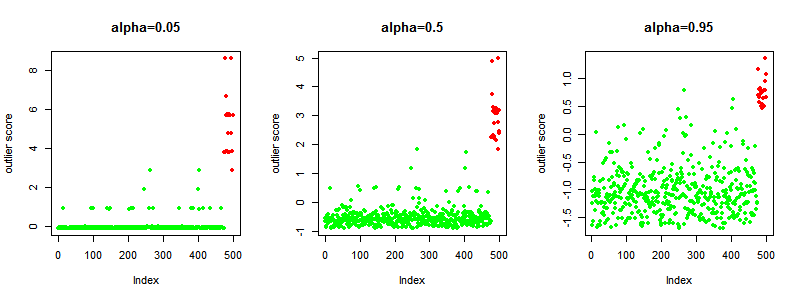
\includegraphics[height=4cm]{outlier_sim1.png}\\
	\label{fig:fig1}
	\caption{Index plots for simulation setup 1 (Left to right) $\alpha = 0.1, 0.5, 0.9$}
\end{figure}

\begin{figure}[t]
	\centering
		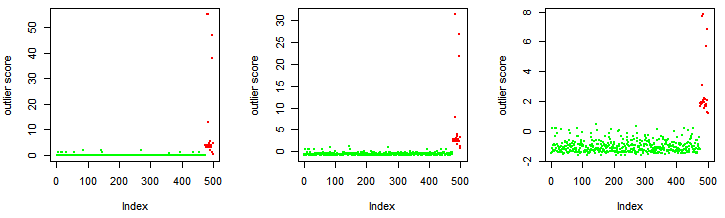
\includegraphics[height=4cm]{outlier_sim2.png}\\
	\label{fig:fig2}
	\caption{Index plots for simulation setup 2 (Left to right) $\alpha = 0.1, 0.5, 0.9$}
\end{figure}

\subsection{Real data examples}

\begin{figure}[t]
	\centering
		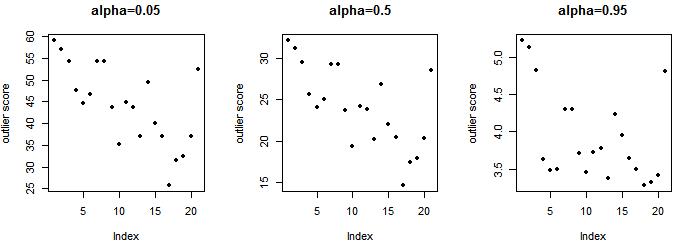
\includegraphics[height=4cm]{outlier_stackloss.png}\\
	\label{fig:fig3}
	\caption{Outlier scores for stackloss data}
\end{figure}

\begin{figure}[t]
	\centering
		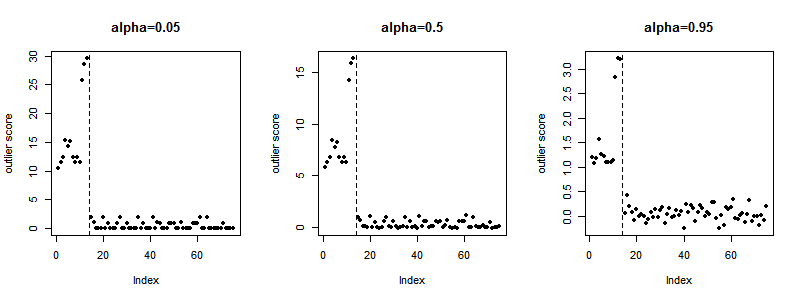
\includegraphics[height=4cm]{outlier_hbk.png}\\
	\label{fig:fig4}
	\caption{Outlier scores for Hawkins-Bradu-Kass data \\(Dotted line at index = 14)}
\end{figure}

\paragraph{Stackloss data}This dataset due to Brownlee [ref] has been widely used for detecting outliers in regression or unsupervised analysis [refs]. It consists of 21 observations in a plant regarding oxidation of Ammonia to Nitric Acid, and has 3 predictors: air flow, cooling temperature and concentration of acid; and percentage of ingoing Ammonia that escapes as response variable. A simple linear regression reveals observation 21 as outlier.

\paragraph{}We set aside the response variable and calculate outlier scores based only the 3 predictor variables. Fig. 3 shows the outlier scores for $\alpha = 0.05, 0.5$ and 0.95. In all the plots the 21st observation is among those with highest outlier scores( especially for $\alpha = 0.95$).

\paragraph{Hawkins, Bradu amd Kass data}This artificial dataset given by Hawkins \textit{et al} [ref] consists of 75 observations and 4 variables (3 predictors and 1 response variable). The first 10 observations are high influential points while observations 11 to 14 are good leverage points. Our analysis using outlier scores based on the 3 predictor variables (Figure 4) identifies all the first 14 observations as outliers.

%\begin{figure}[t]
%	\centering
%		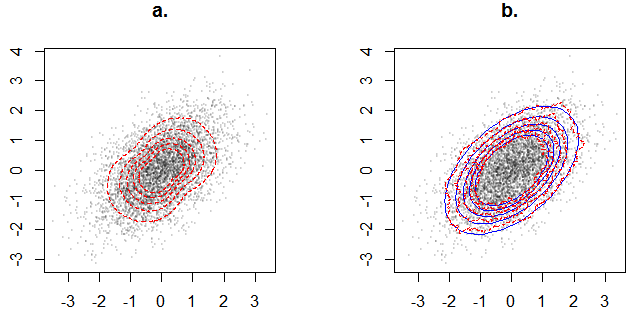
\includegraphics[height=5cm]{Sim_bvn.png}\\
%		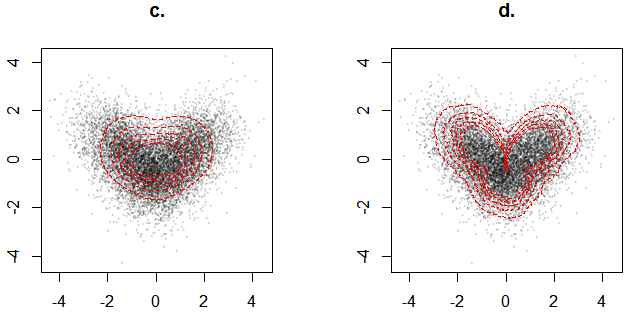
\includegraphics[height=5cm]{Sim_mixsym.png}\\
%		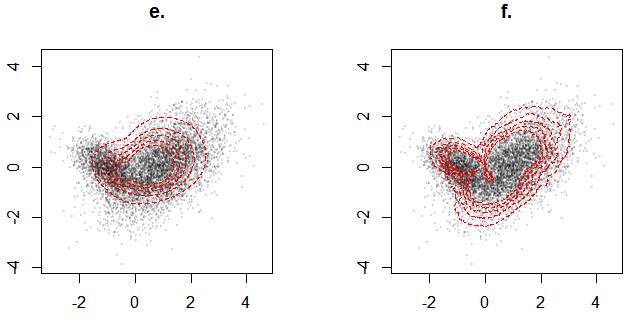
\includegraphics[height=5cm]{Sim_mixasym.png}\\
%		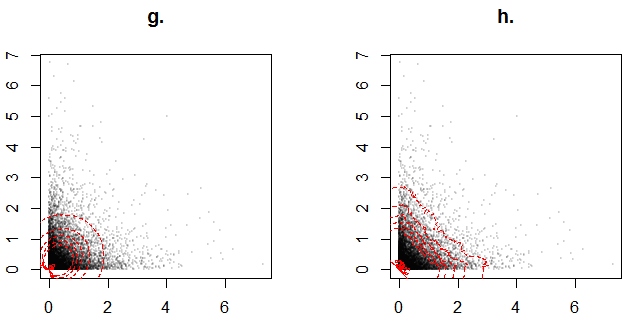
\includegraphics[height=5cm]{Sim_exp2.png}
%	\label{fig:fig1}
%	\caption{(Left) PQ and (Right) WPQ profiles for the four simulation scenarios. Blue lines in panel b represent actual confidence ellipsoids}
%\end{figure}
\end{document}